\section{Experiments} \label{sec:experiments}
	
	In this section the conducted experiments are motivated and presented.
	Therefore, we first present the graph datasets used for the l-WWLLT distance learning (section \ref{subsec:datasets}).
	Then the general setup of the implemented method is explained (section \ref{subsec:exp_setup}).
	We summarize the most important parameters, and how different settings were combined.
	Note that some parameters significantly change the behavior of the implemented method and are primarily used for the research on what specific approach may produce the desired results.
	Further note, that the number of parameters was to great, to allow for an extensive grid search.
	Instead, a few guiding experiments are presented (section \ref{subsec:experiments}).
	More evaluations can be found in the appendix (appendix \ref{Appendix:FurtherResults}).

	192 different experiments on 17 different datasets were conducted using the final implementation of the l-WWLLT method.
	Since at first suitable parameter configurations were unknown, many of these experiments are spot checks for some parameter configurations.
	No extensive gird search was performed for all parameter combinations.
	No reliable trend in performance could be discovered for all datasets.
	That is why in this section we consider sets of experiments and discuss their implications for the research on the l-WWLLT method.
	In section \ref{sec:results} the best results over all computations are briefly summarized and presented.
		
	\subsection{Datasets} \label{subsec:datasets}
		For the experiments, three major sources for datasets of classified graphs were used.
		The TUDataset~\cite{2020_Morris_CONF} and versions of its graph datasets~\cite{2019_Ivanov_CONF}\footnote{\url{https://github.com/nd7141/graph_datasets}}
		and the OGB dataset~\cite{2020_Hu_CONF}.
		The versions of the TUDataset are based on the research by \citeauthor{2019_Ivanov_CONF} and can be seen as a pre-processing of the TUDatasets.
		Since these dataset version have the same names as the original datasets in the TUDataset, we refer to them by adding \enquote{\_c} as a suffix to the original name (see for example table \ref{tab:BestSVM_results}).
		Sine the results between these different versions of the datasets did not reveal substantial insight on the l-WWLLT method with respect to the research question, we do not go into further detail about their construction here.
				
		All loaded datasets were pre-processed, to ensure equalized treatment between the different sources, and to discard not needed information.
		This includes the deletion of graphs without vertices (where the WL-labeling is not applicable) and adding uniform vertex labels, if none are present.
		Furthermore the practical implementation converts the graphs into a standardized format consisting of only a vertex set with vertex labels, and an edge set.
		Since these practical implementation choices do not effect the theoretical reasoning and the l-WWLLT method itself, we do not discuss them in detail in this thesis.
		
		\subsubsection{TU Dataset} \label{subsec:TUDataset}
			
			The increased need of benchmark graph classification datasets lead to the construction of a graph dataset collection at TU Dortmund~\cite{2016_Kersting_CONF, 2020_Morris_CONF}.
			We refer to these datasets as TUDatasets.
			\citeauthor{2021_Schulz_CONF} argued, that these datasets may not be sufficient to test graph classification datasets, since good classification accuracy can be achieved by discarding a lot of structural information on the graphs (recall section \ref{subsec:comparison_to_other_methods}).
			Furthermore these datasets contain only $200$ to $5,000$ graphs, which may be to small for meaningful tests of graph kernels on classification tasks~\cite{2021_Schulz_CONF}.
			See table \ref{tab:TUDataset_Stats} for more information on the datasets.\footnote{*The dataset \textit{Tox21\_AhR} is also called \textit{Tox21\_AhR\_training}.}.
			However, because these datasets have been used by many other researchers and allow for a faster test driven development of the l-WWLLT method, we also use them for to evaluate the method as well (for example \cite{2007_Wale_CONF, 2016_Kriege_NIPS, 2011_Shervashidze_JMLR, 2015_Yanardag_CONF, 2020_Siglidis_CONF, 2020_Dwivedi_CONF, 2021_Schulz_CONF}).
			
			\begin{table}[H]
				\centering
				\begin{tabular}{|l|l|l|l|l|l|}
					\hline
					\textbf{Dataset} & \textbf{Source} & \textbf{\#Graphs} & \textbf{\#Classes} & \textbf{Avg. $|V|$} & \textbf{Avg. $|E|$} \\ \hline
					\multicolumn{6}{|c|}{\textbf{Small molecules}} \\ \hline
					\textbf{AIDS} & ~\cite{2008_Riesen_CONF, URL_TUDataset_NCI} & 2000 & 2 & 15.69 & 16.20 \\ \hline
					\textbf{MUTAG} & ~\cite{1991_Debnath_CONF, 2012_Kriege_CONF} & 188 & 2 & 17.93 & 19.79 \\ \hline
					\textbf{NCI1} & ~\cite{2007_Wale_CONF, 2011_Shervashidze_JMLR} & 4110 & 2 & 29.87 & 32.30 \\ \hline
					\textbf{NCI109} & ~\cite{2007_Wale_CONF, 2011_Shervashidze_JMLR} & 4127 & 2 & 29.68 & 32.13 \\ \hline
					\textbf{PTC\_MR} & ~\cite{2001_Helma_CONF, 2012_Kriege_CONF} & 344 & 2 & 14.29 & 14.69 \\ \hline
					\textbf{Tox21\_AhR}* & ~\cite{URL_TUDataset_Tox21} & 8169 & 2 & 18.09 & 18.50 \\ \hline
					\multicolumn{6}{|c|}{\textbf{Bioinformatics}} \\ \hline
					\textbf{DD} & ~\cite{2011_Shervashidze_JMLR} & 1178 & 2 & 284.32 & 715.66 \\ \hline % \cite{2003_Dobson_CONF}
					\textbf{ENZYMES} & ~\cite{2005_Borgwardt_CONF} & 600 & 6 & 32.63 & 62.14 \\ \hline % 2004_Schomburg % https://academic.oup.com/nar/article/32/suppl_1/D431/2505276?login=true
					\textbf{PROTEINS} & ~\cite{2005_Borgwardt_CONF} & 1113 & 2 & 39.06 & 72.82 \\ \hline % , 2003_Dobson_CONF
					\multicolumn{6}{|c|}{\textbf{Computer vision}} \\ \hline
					\textbf{MSRC\_9} & ~\cite{2015_Neumann_SPRINGER} & 221 & 8 & 40.58 & 97.94 \\ \hline
					\textbf{MSRC\_21} & ~\cite{2015_Neumann_SPRINGER} & 563 & 20 & 77.52 & 198.32 \\ \hline
					\textbf{MSRC\_21C} & ~\cite{2015_Neumann_SPRINGER} & 209 & 20 & 40.28 & 96.60 \\ \hline
				\end{tabular}
				\caption{Statistics on some TUDatasets}\label{tab:TUDataset_Stats}
			\end{table}			

			The TUdatasets are based on different graphs representing different data structures.
			For example, the \textit{MUTAG} dataset contains 188 graphs, depicting chemical compounds.
			In this representation, explicit hydrogen atoms have been removed. 
			The (initial) vertex labels stand for example atoms like for Carbon (0), Nitrogen (1), Oxygen (2), Fluorine (3), Iodine (4), Chlorine (5) and Bromine (6).
			The edges labels indicate the bond type of either aromatic (0), single (1), double (2) or triple (3).
			The classifications in this dataset are made according to their mutagenic effect on a bacterium~\cite{1991_Debnath_CONF}.

			Note that most, but not all, of these datasets have two class labels and that datasets with high amounts of different class labels require bigger batch sizes in order to represent all classes equally.
			More information on the individual datasets can be found online.\footnote{TUDataset list \url{https://chrsmrrs.github.io/datasets/docs/datasets/}}
															
		\subsubsection{OGB Dataset} \label{subsec:OGB}
			
			As mentioned above, the TUDatasets may not be ideal to test graph classification kernels.
			Thus there is a high demand for graph datasets where the graph classification is highly dependent on the graph structure.			
			In 2020 \citeauthor{2020_Hu_CONF} presented the Open Graph Benchmark (OGB)~\cite{2020_Hu_CONF}.
			This collection includes large-scale datasets from different domains and for different applications, such as vertex, link, and graph property predictions.
			The datasets are grouped into datasets with small (100 thousand to 1 million vertices), medium (>1 million vertices) and large (on the order of 100 Mio. vertices or 1 billion edges) graphs~\cite{2020_Hu_CONF}.
					
			The datasets \textit{ogbg-molhiv} and \textit{ogbg-molpcba} were initially considered for experimentation.
			But their size of 41,127 and 437,929 graphs was to big (with respect to RAM storage) to experiment on various configuration settings.
			Notice that for the evaluation, the distance matrix (and kernel matrix) is computed for every learned and stored edge weight vector.
			It is possible to continue the evaluation on a fraction of the matrices, or fractions of the datasets.
			Instead, the experiments were focused on smaller datasets from this framework, in order to execute and learn from more experiments.
			The OGB collection provides ten smaller datasets from MoleculeNet~\cite{2018_Wu_CONF}.
			However of those, only the datasets \textit{ogbg-molbace} and \textit{ogbg-molbbbp} match the requirements of samples for binary (not multi-task) classifications.
									
			The leaderboard\footnote{\url{https://ogb.stanford.edu/docs/leader_graphprop/\#ogbg-molhiv}} of classification performance on these datasets is organized by ROC-AUC (Receiver Operating Characteristics-Area Under The Curve) scores.
			This quality measurement and evaluation process was not introduced to the implemented method for this thesis and thus the evaluation on these two datasets from the OGB collection was not compared to the state of the art.
			This decision is justified by the desire to avoid introducing yet another evaluation strategy and because these two datasets were loaded and pre-processed differently than how the OGB framework proposes it.			
			Instead, these datasets are used only to track the performance against the l-WWLLT metric at its initialization, as described in the research question (section \ref{subsec:research_question}). 
			
	\subsection{Set Up} \label{subsec:exp_setup}
	
		For all experiments a few parameter settings were kept fixed.
		One may very them in later research.
		These parameters are the update frequency, -score and -intensity.
		For all experiments, the \textbf{update frequency} is set to \enquote{epoch}, which means that the edge weights were updated after computing the mean weight change for all edges and all graphs in the batch of one epoch. 
		For all experiments the \textbf{update scope} is set to \enquote{All layers equal}, which means that all layers are treated equally. One may use this parameter to change the update intensity for individual layers individually.
		
		The implemented Edge Weight Learner (as explained in section \ref{subsec:EWL}) has a few more parameters, whose values were changed during the experimentation phase.	
		Starting with the \textbf{WLLT depth} $D$, which refers to the deepest layer of the WLLT whose edge weights are changed.
		If it is set to $D=2$ only the edge weights of the layers $0$, $1$ and $2$ are updated (and used to define the update).
		The \textbf{learning rate} $lr$ refers to an adjustment parameter, typical for machine learning (section \ref{subsec:EWL}).
		The \textbf{batch size} $bs$ is the percentage of graphs of the whole dataset that are used for adjusting the edge weights in one epoch.
		Notice that the actual set of graphs for each epoch is determined before all epochs, such that each class is represented almost equally.
		The \textbf{push factor} ($f_{\text{push}}$), \textbf{pull factor} ($f_{\text{pull}}$) and \textbf{Heaviest Earth Threshold} ($t_{\text{he}}$) refer to the same parameters explained in section \ref{subsec:EWL}.
		The flag \textbf{$w\in[0,2]$} (or $w\notin[0,2]$) indicates, if all edge weights were limited to the interval $[0, 2]$. 
		The motivation for this parameter is explained in section \ref{subsubsec:exp_WeightLimit}.
		Notice that this can be understood as an upper boundary ($w\le 2$), since the edge weights are always kept non-negative anyways.
					
		All experiments were implemented in Python 3.7.7.
		The few reported runtimes were measured using an Intel Core i5-8300 CPU at 2.30GHz with 16GB of RAM using a single processor only.
	
\subsection{Experiments} \label{subsec:experiments}
		
	First experiments were conduced to guide implementation choices and sha\-pe the evaluation process.
	This includes not only the evaluation with respect the proposed SVM and cluster scores, but also with respect to tracking and visualizing the computed edge weights and the resulting clustering.
	Most of these evaluations are used and presented in the next sections about the experiments.
	
	
	\subsubsection{Batch Size, WLLT Depth and Number of Epochs} \label{subsubsec:exp_eopchs}
	
		\paragraph{Batch Size} The number of epochs is closely related to the batch size in the sense that both parameters relate positively to the possibilities of introduced or removed weight in the WLLT.
		However the batch size goes quadratically into the runtime and thus should kept low if possible.
		Furthermore, the evaluation and the application of the weight updates is performed after batch, a smaller batch size allows for a finer evaluation.
		That is why in general the batch size was kept at 50 to 200 graphs ($1\%$-$30\%$) for the datasets, depending on the size of the dataset and sizes of the graph classes.
		Examples are presented in tabular \ref{tab:BestSVM_results}.
		
		\paragraph{WLLT Depth} The depth of the WLLT has a significant impact on the runtime (and on the required storage) as well.
		Although as discussed, the size of the WLLT has linear effect on the runtime, the WLLT depth may have exponential effect on the WLLT size and thus the runtime.
		That is because the amount of WL-labels increases drastically, depending on the dataset (recall figures \ref{fig:plotwlltl2e0aids2915h-25m} and \ref{fig:plotwlltmutagl2}).
		Table \ref{tab:WLLTsize} in the appendix (\ref{Asub:WLLTStatistics}) lists the WLLT size up to layer four for a selection of datasets.
		Figure \ref{fig:wlltstatsallds} visualizes this table.
		
		\begin{figure}[H]
			\centering
			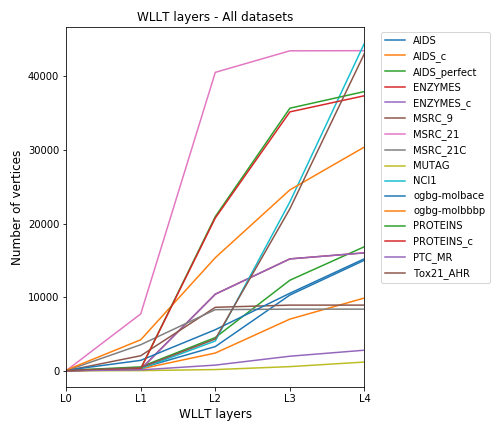
\includegraphics[width=0.7\linewidth]{images/WLLTstats_AllDs}
			\caption{Size of the WLLTs for various datasets.}
			\label{fig:wlltstatsallds}
		\end{figure}		
		
		Consider a graph representation of a graph $G$, and a WL-label $l$ which is a leaf in the WLLT and does not occur in the labelings for $G$.
		Since $l$ is present in the WLLT, it is present in the dataset and adding a next WLLT layer adds at least one child vertex to $l$.
		Depending on the depth and the dataset, $l$ may get many more children and all these do not occur in the labeling for $G$ as well.
		Thus notice, how higher layers imply a more sparse graph representation.
		After conducting some initial experiments with smaller datasets for WLLT depths of up to $10$, the WLLT depth was kept at $3$ or $4$.
		Higher layers do not seem to improve the resulting similarity measure significantly or at all.
		
		\paragraph{Number of Epochs} To determine how many epochs a learning algorithm should perform is usually related to the task of detecting over-fitting.
		For efficiency reasons, the evaluation and the learning procedure were separated, which is why an automatic detection of over-fitting was not implemented.
		Instead, the experiments were focused on collecting data for several parameter settings, and possibly detect over-fitting in hindsight.
		For a more granular evaluation the implementation saves intermediate results (a weight vector for the WLLT) every $10$-th epoch.
		
		The highest number of epochs was 1000.
		For the dataset \textit{AIDS} with 100 graphs per batch this took approximately 7.5 seconds per epoch (75 milliseconds per batch) and a total runtime of approximately two hours.
		The overall performance of the learned similarity measure did not show a clear relation (improvement or degeneration) with the number of epochs.
		Since all evaluations show noticeable development in the first $200$ epochs, this was used as the standard number of epochs for further experiments.
		See figure \ref{fig:plota1massevalscorecalinski} for example. 
		The visualized Calinski-Harabasz cluster score only changes significantly for the dataset \textit{PROTEINS\_c}.
		All other trajectories of the plots were maintained for most of the experiments for further learning epochs.
		No clear relation to other performance criteria (e.g. SVM accuracy or SME) of the l-WWLLT was detected.
		
		\begin{figure}[H]
			\centering
			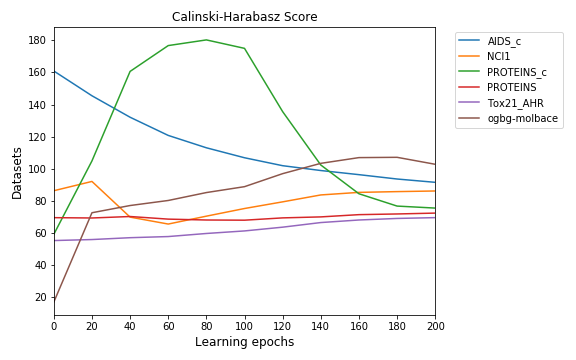
\includegraphics[width=\linewidth]{images/plotA1_MassCHS.png}
			\caption{Calinski-Score for several different datasets.}
			\label{fig:plota1massevalscorecalinski}
		\end{figure}
		
		The following plots for the dataset \textit{ogbg-molbace} are exemplary visualizations for this observation.
		They correspond to a run with learning epochs $e=500$, WLLT depth $D=5$, batch size of 100 graphs, learning rate $lr=1.0$ and push and pull factors of $0.2$ each with limited edge weight in the interval $[0,2]$ (figures \ref{fig:InterMeanMinMolBrace}, \ref{fig:IntraMeanMaxDistMolBace}, \ref{fig:plota1totalweightsumogbgmolbaceexp1}, \ref{fig:plota1scoresilhouetteogbgmolbaceexp1}, \ref{fig:plota1scoredaviesbouldinogbgmolbaceexp1}, \ref{fig:plota1scorecalinskiharabaszogbgmolbaceexp1}, and \ref{fig:plota1maxwplogbgmolbaceexp1}).
		
		\begin{figure}[!ht]
			\centering
			\begin{subfigure}{0.49\textwidth}
				\centering
				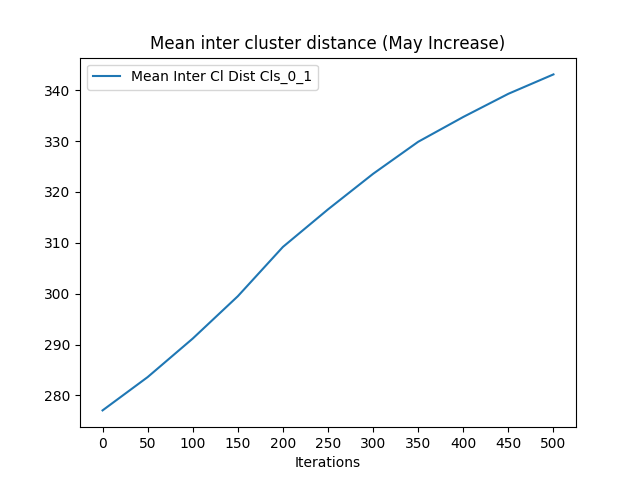
\includegraphics[width=1.1\linewidth]{images/plotA1_InterMeanClDist_ogbgMolbaceExp1}
				\caption{Mean cluster distance}
				\label{fig:plota1intermeancldistogbgmolbaceexp1-25m}
			\end{subfigure}
			\begin{subfigure}{0.49\textwidth}
				\centering
				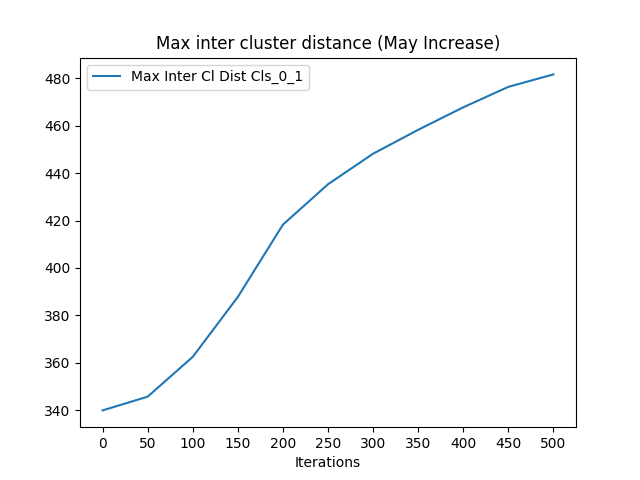
\includegraphics[width=1.0\linewidth]{images/plotA1_InterMaxClDist_ogbgMolbaceExp1}
				\caption{Maximum cluster distance}
				\label{fig:plota1intermaxcldistogbgmolbaceexp1}
			\end{subfigure}
			\caption{Mean and Maximum cluster distances - \textit{ogbg-molbace}}
			\label{fig:InterMeanMinMolBrace}
		\end{figure}
		
		The dataset \textit{ogbg-molbace} contains graphs, which are grouped into two clusters ($0$ and $1$).
		The two plots in figure \ref{fig:InterMeanMinMolBrace} show the mean and maximum distance between these classes (inter-distance).
		As desired, these distances increase over time.
		Round epoch 200, a slightly but rather insignificant reduced growth of the maximum distance can be noticed.		
		
		\begin{figure}[!ht]
			\centering
			\begin{subfigure}{0.49\textwidth}
				\centering
				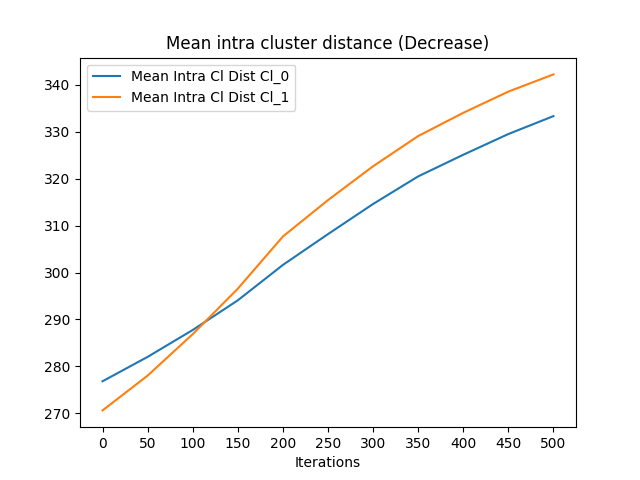
\includegraphics[width=1.1\linewidth]{images/plotA1_IntraMeanClDist_ogbgMolbaceExp1}
				\label{fig:plota1intrameancldistogbgmolbaceexp1}
			\end{subfigure}
			\begin{subfigure}{0.49\textwidth}
				\centering
				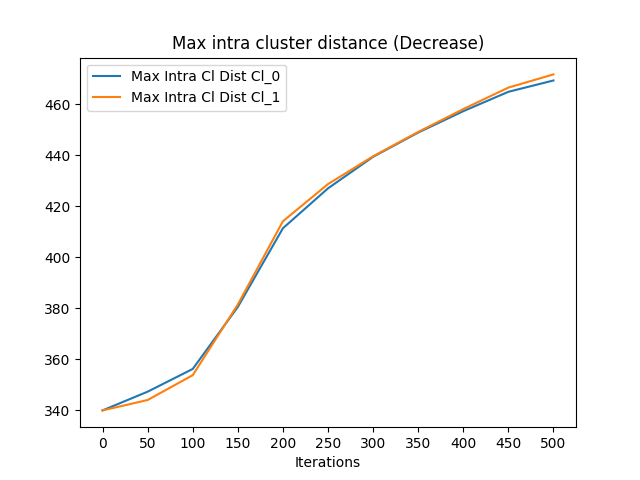
\includegraphics[width=1.1\linewidth]{images/plotA1_IntraMaxClDist_ogbgMolbaceExp1}
				\label{fig:plota1intramaxcldistogbgmolbaceexp1}
			\end{subfigure}
			\caption{Intra-cluster statistics - \textit{ogbg-molbace}}
			\label{fig:IntraMeanMaxDistMolBace}
		\end{figure}
		
		The two plots in figure \ref{fig:IntraMeanMaxDistMolBace} show the mean and maximum distance between samples of the same class each (intra-distance).
		Again around epoch 200, the reduced growth of the maximum distance can be noticed.
		One may as well describe it as a significant increase in the epochs 100 to 200.
		In contrast to the distances between different clusters however, the desired behavior would be decreasing intra-distances instead.
		Also notice that the order of magnitudes are equal to the inter-distances.
		
		\begin{figure}[H]
			\centering
			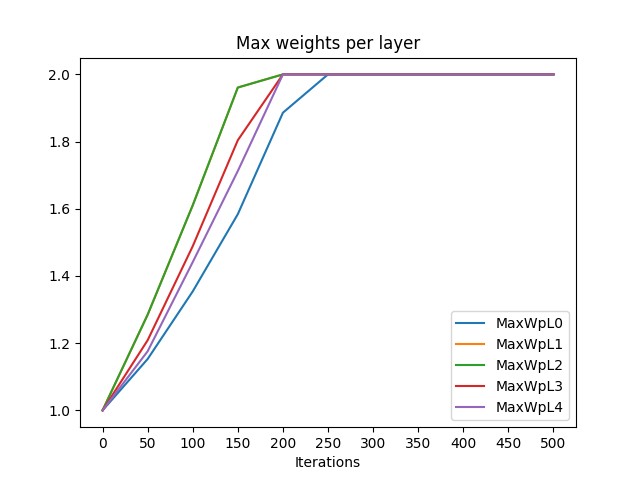
\includegraphics[width=0.7\linewidth]{images/plotA1_MaxWpL_ogbgMolbaceExp1}			
			\caption{Maximum weights per WLLT layer - \textit{ogbg-molbace}}
			\label{fig:plota1maxwplogbgmolbaceexp1}	
		\end{figure}
		
		The plot in figure \ref{fig:plota1maxwplogbgmolbaceexp1} gives a good explanation for the observed statistics up to epoch 200.
		It shows the maximum edge weights, to each of the five layers in the WLLT.
		Around epoch 200 the maximum edge weight for every epoch has reached the allowed limit, and stays there.
		Recall, that the update rule may treat weights of the same value equally.
		One may assume, that after epoch 200 more and more edge weights are set to the maximum of $2.0$ and no longer decreased.
		
		\begin{figure}[H]
			\centering
			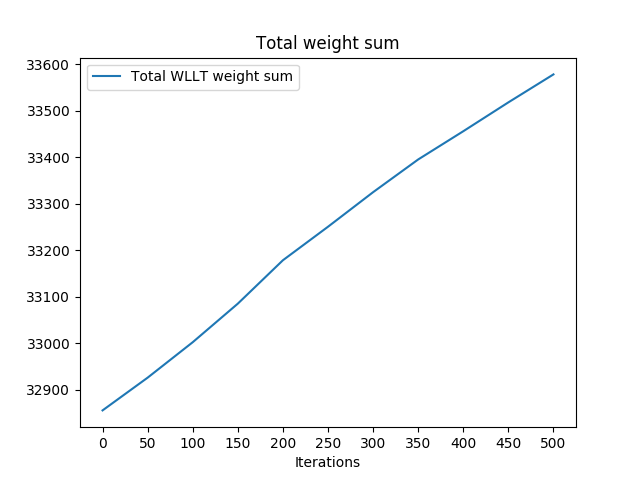
\includegraphics[width=0.7\linewidth]{images/plotA1_TotalWeightSum_ogbgMolbaceExp1}
			\caption{Total WLLT weight - \textit{ogbg-molbace}}
			\label{fig:plota1totalweightsumogbgmolbaceexp1}
		\end{figure}			
		
		These observations are supported by figure \ref{fig:plota1totalweightsumogbgmolbaceexp1}, which shows that the overall weight in the WLLT grows monotonically.
				
		\begin{figure}[H]
			\centering
			\begin{subfigure}{0.3\textwidth}
				\centering
				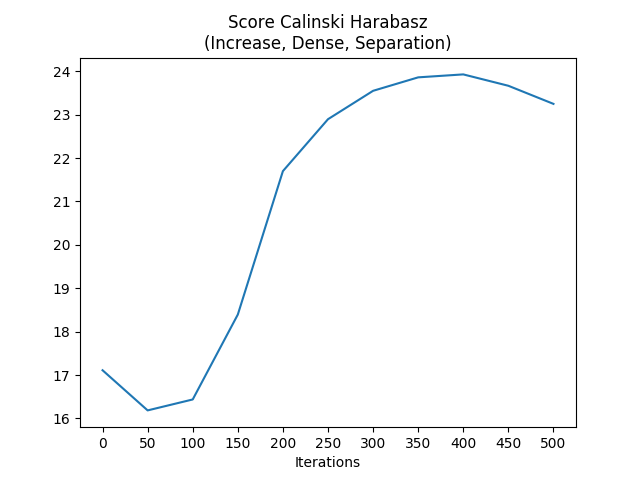
\includegraphics[width=1.1\linewidth]{images/plotA1_Score_Calinski_Harabasz_ogbgMolbaceExp1}
				\caption{CHS}
				\label{fig:plota1scorecalinskiharabaszogbgmolbaceexp1}
			\end{subfigure}		
			\begin{subfigure}{0.3\textwidth}
				\centering
				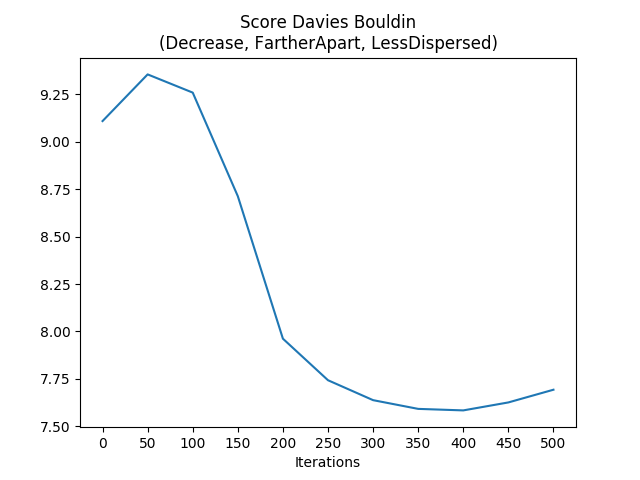
\includegraphics[width=1.1\linewidth]{images/plotA1_Score_Davies_Bouldin_ogbgMolbaceExp1}
				\caption{DBS}
				\label{fig:plota1scoredaviesbouldinogbgmolbaceexp1}
			\end{subfigure}
			\begin{subfigure}{0.3\textwidth}
				\centering
				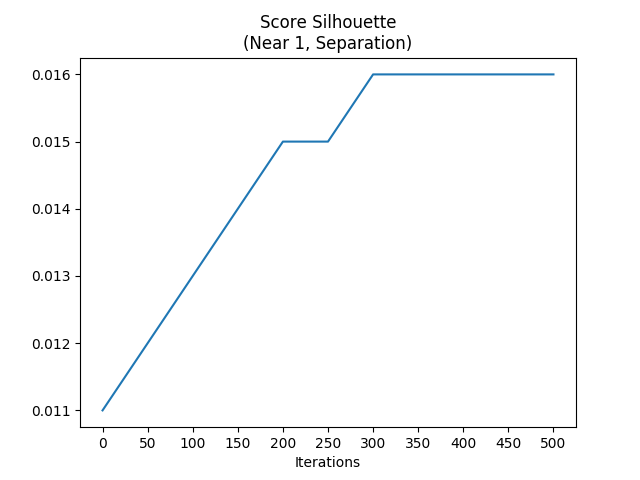
\includegraphics[width=1.1\linewidth]{images/plotA1_Score_Silhouette_ogbgMolbaceExp1}
				\caption{SS}
				\label{fig:plota1scoresilhouetteogbgmolbaceexp1}
			\end{subfigure}
			\caption{Cluster scores - \textit{ogbg-molbace}}
			\label{fig:ClScores_molbace}
		\end{figure}
				
		The cluster scores (see figures \ref{fig:ClScores_molbace}) indicate, that this edge weight maximum reduced the quality of the clustering.
		After epoch 200 all three scores indicate a reduced improvement and even degeneration.
		Recall, that the Calinski-Harabasz Score corresponds to the denseness of the clusters and their separation.
		Its improvement can be traced to the improved separation.
		The analogue situation can seen in the plot of the Davies-Bouldin score.
		The Silhouette Score stagnates after epoch 300 (at a low level).
		Since it corresponds to the separation, and not directly to the denseness of the clusters, one can deduce, that the degeneration of the other two scores can be explained by a degeneration of the cluster denseness.
		Combined with the insight from figure \ref{fig:plota1maxwplogbgmolbaceexp1} we can deduce, that the chosen setting leads to a reliable increase of the inter-distances, but not of the intra-distances and thus decreases the denseness of the clusters.
		
		\begin{figure}[H]
			\centering
			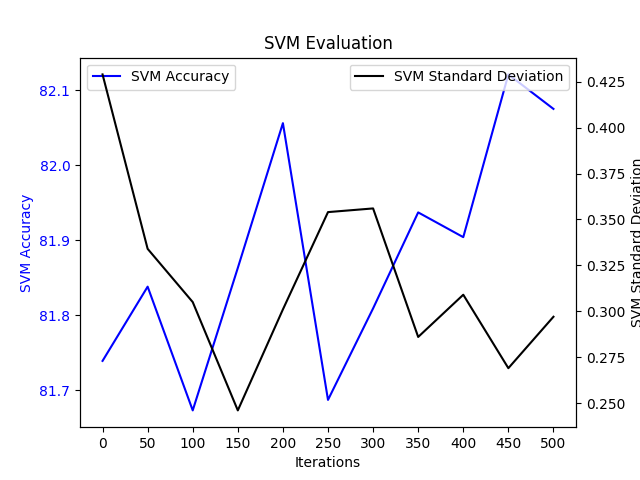
\includegraphics[width=0.7\linewidth]{images/plotA1_SVM_ogbgMolbaceExp1}
			\caption{SVM accuracy and standard deviation}
			\label{fig:plota1svmogbgmolbaceexp1}
		\end{figure}
		
		Interestingly, the SVM accuracies (shown in figure \ref{fig:plota1svmogbgmolbaceexp1}) do not obviously relate to the other plots.
		The SVM accuracy fluctuates at almost $82\%$.
	
	\subsubsection{Edge Weight Limit} \label{subsubsec:exp_WeightLimit}
		
		The initial configuration of the implemented learner did not include an edge weight limit.
		However the drawbacks of the multiplicative updates, in the context of the WLLT and the graph representations can be seen in the plots in figure \ref{fig:MUTAG_exponential_layers}.
		Each plot shows the edge weight distribution over all its WL-labels for all 500 learning epochs.
		The x-axes denote the WL-label (child to the considered edge), the y-axes the learning epoch and the z-axes the edge weights.
		The plots visualize how the (non-zero) development of most edge weights is overshadowed by an exponential growth of a few weights.
				
		\begin{figure}[H]
			\centering
			\begin{subfigure}{0.3\textwidth}
				\centering
				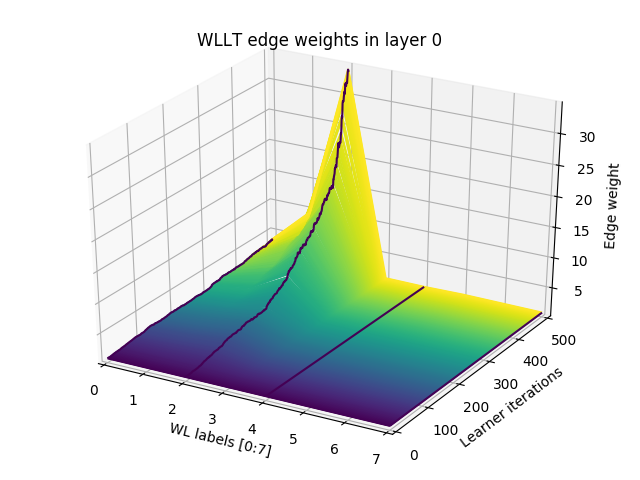
\includegraphics[width=1.\linewidth]{images/plotA3_WLLT_ewL0_MUTAG_d5_e500}
				\caption{Layer 0}
				\label{fig:fig:plota3wlltewl0mutagd5e500}
			\end{subfigure}		
			\begin{subfigure}{0.3\textwidth}
				\centering
				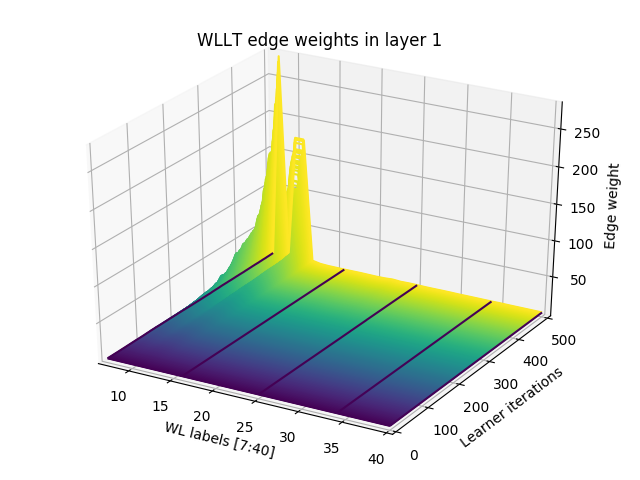
\includegraphics[width=1.\linewidth]{images/plotA3_WLLT_ewL1_MUTAG_d5_e500}
				\caption{Layer 1}
				\label{fig:fig:plota3wlltewl1mutagd5e500}
			\end{subfigure}
			\begin{subfigure}{0.3\textwidth}
				\centering
				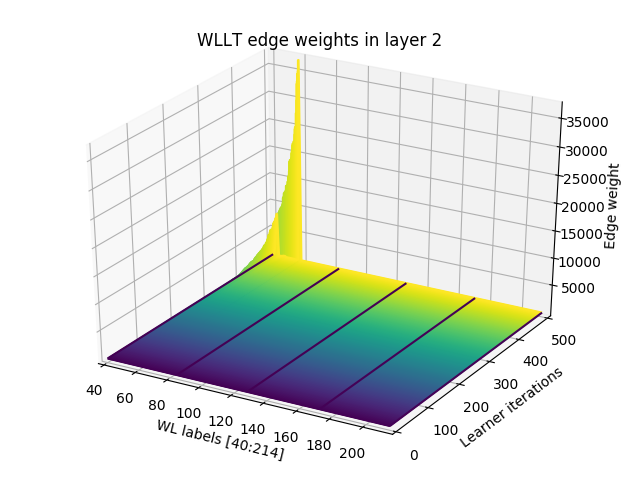
\includegraphics[width=1.\linewidth]{images/plotA3_WLLT_ewL2_MUTAG_d5_e500}
				\caption{Layer 2}
				\label{fig:fig:plota3wlltewl2mutagd5e500}
			\end{subfigure}
			\caption{Edge weights per WLLT layer - \textit{MUTAG}}
			\label{fig:MUTAG_exponential_layers}
		\end{figure}
	
		These and similar experiments show, that the same edge weights are updated predominantly in the same direction (mostly increased or mostly decreased).
		Thus by nature of the relative updates, some weights may increase exponentially.	
		A weight limit (to the interval $[0,2]$) was introduced in order to reduce this overshadowing effect and keep the edge weight values reasonable.
		The effect, that only a few edge weights are updated most frequently and strongly remains, and is discussed in the following paragraph.
			
		\paragraph{Redemption of unlimited Weights} The idea was, to limit the edge weights to the interval $[0, 2]$.
		As we can see in the descriptions of the other experiments, it was difficult to find a configuration for the implementation, such that the edge weights do not clip to the imposed ceiling and also do not vanish.
		Both results were observed.
		A grid search for the values $0.05$, $0.1$, $0.3$, $0.5$, $1.0$ was performed.
		While the learning rate varied between $1.0$, $0.9$ and $0.5$.
		No reliable improving configuration was found and the edge weight adjustment may have been to big throughout the grid search.
		This assumption can be supported by a rather positive result, when lifting the edge weight constraints on a learning setting with different parameters.		
				
		The plots in figure \ref{fig:MaxMeanWpL_AIDS} show how the maximum edge weight and the mean edge weight grow exponentially in the number of learning epochs.
		Similarly, the plots in figure \ref{fig:EWWireframe_AIDS} highlight the domination of individual edge weights in the layers $0$ and $1$.
		These wire-frame plots are a great tool to compare the development of all edge weights per layer.
		Noticeable in all experiments is, that in all layers, the total weight is concentrated on a small portion of WL-labels.
		These are the most common WL-labels and dominate the graph representations, especially in the lower layers.
		With each layer, the differentiation of the WLLT vertices (their WL-labels and thus the represented $k$-th neighborhoods) increases monotonically and the frequencies of all WL-labels decreases.
		Accordingly, the strength of the update rule on these WL-labels decreases.
		The domination of the weight of the \enquote{lowest edge} in figure \ref{fig:EWWireframe_AIDS} however, is unusually high, due to its exponential increase.
		
		\begin{figure}[H]
			\centering	
			\begin{subfigure}{0.45\textwidth}
				\centering
				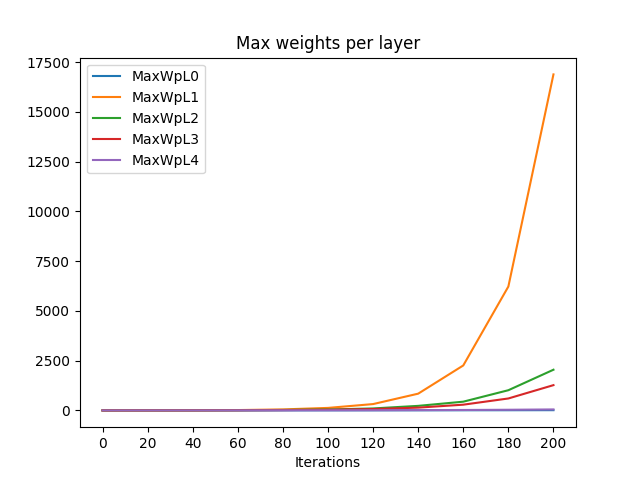
\includegraphics[width=1.1\linewidth]{images/plotA2_MaxWpL_AIDS_GDL_24_17h-05}
				\caption{MaxWpl}
				\label{fig:plota2maxwplaidsgdl2417h-05}
			\end{subfigure}
			\begin{subfigure}{0.45\textwidth}
				\centering
				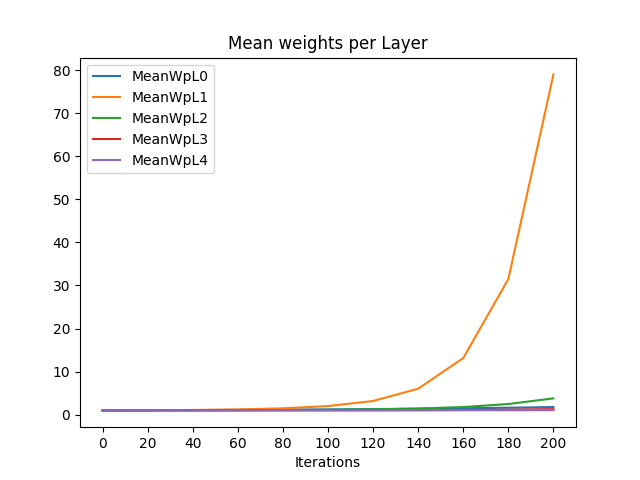
\includegraphics[width=1.1\linewidth]{images/plotA2_MeanWpL_AIDS_GDL_24_17h-05}
				\caption{MeanWpl}
				\label{fig:plota2meanwplaidsgdl2417h-05}
			\end{subfigure}
			\caption{Maximum and mean weights per layer - \textit{AIDS}}
			\label{fig:MaxMeanWpL_AIDS}
		\end{figure}
		
		
		\begin{figure}[H]
			\centering	
			\begin{subfigure}{0.45\textwidth}
				\centering
				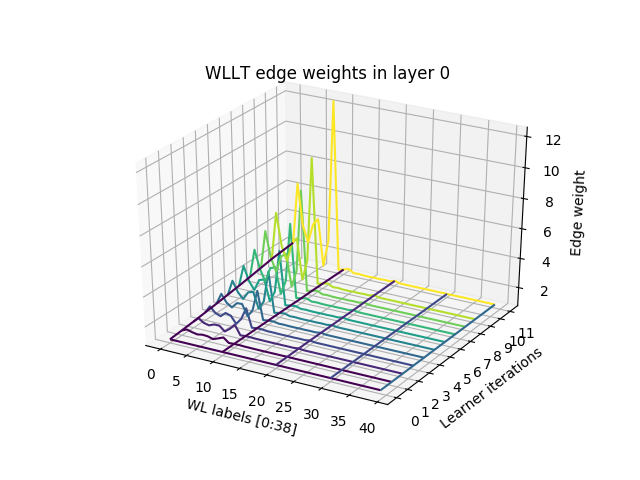
\includegraphics[width=1.1\linewidth]{images/plotA2_WLLTL0_AIDS_GDL_24_17h-05}
				\caption{Layer 0}
				\label{fig:plota2wlltl0aidsgdl2417h-05}
			\end{subfigure}
			\begin{subfigure}{0.45\textwidth}
				\centering
				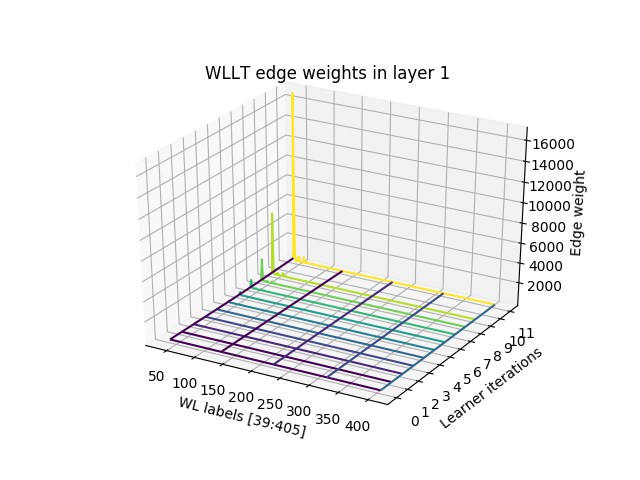
\includegraphics[width=1.1\linewidth]{images/plotA2_WLLTd1_AIDS_GDL_24_17h-05}
				\caption{Layer 1}
				\label{fig:plota2wlltd1aidsgdl2417h-05}
			\end{subfigure}
			\caption{Edge weights per layer, per iteration - \textit{AIDS}}
			\label{fig:EWWireframe_AIDS}
		\end{figure} 
		
		Despite this exponential edge weight increase, which was deemed undesirable in the early experiments, the evaluation shows how the SVM accuracy improves in this setting.
		The exponentially increasing total weight in the WLLT, shown in figure \ref{fig:plota2totalweightsumaidsgdl2417h-05} and the almost strictly monotonically improving SVM accuracy in figure \ref{fig:plota2svmaidsgdl2417h-05} indicate, that more research on different settings need to be considered.
		We also can conclude a positive answer of the research question from this result.
		However more experiments are required, do identify configuration strategy to obtain such improvements.
		
		\begin{figure}[H]
			\centering	
			\begin{subfigure}{0.45\textwidth}
				\centering
				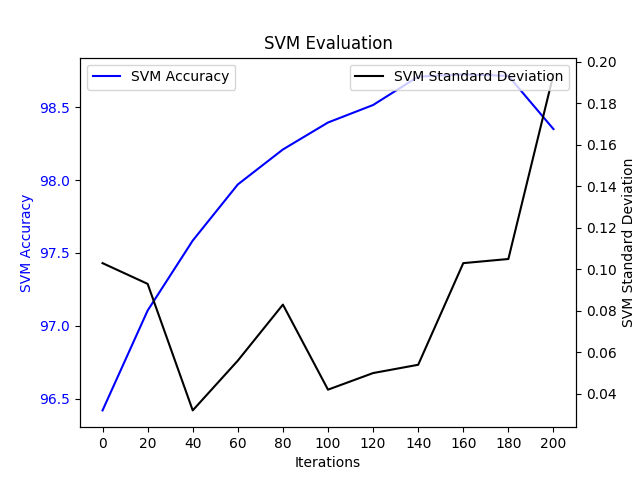
\includegraphics[width=1.1\linewidth]{images/plotA2_SVM_AIDS_GDL_24_17h-05}
				\caption{SVM}
				\label{fig:plota2svmaidsgdl2417h-05}
			\end{subfigure}
			\begin{subfigure}{0.45\textwidth}
				\centering
				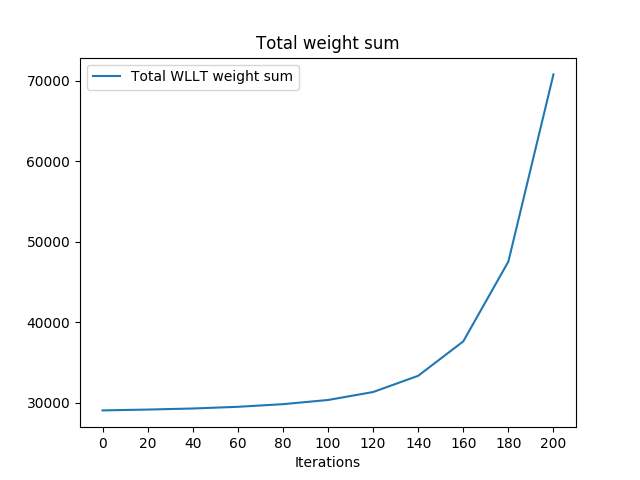
\includegraphics[width=1.1\linewidth]{images/plotA2_TotalWeightSum_AIDS_GDL_24_17h-05}
				\caption{Total weight sum}
				\label{fig:plota2totalweightsumaidsgdl2417h-05}
			\end{subfigure}
			\caption{SVM and total weight sum - \textit{AIDS}}
			\label{fig:SVMTotalWS_AIDS}
		\end{figure}	
	
	\subsubsection{Artificial Dataset} \label{subsubsec:exp_AIDS_perfect}
		
		To test the correctness of the implemented method an artificial dataset was created.
		This dataset shall represent a perfect separation of the classes with respect to the l-WWLLT with uniformly initialized edge weights.
		Therefore the 2000 graphs of the dataset \textbf{AIDS} were subdivided in class $A$, consisting of the first thousand graphs and class $B$, consisting of the second thousand graphs.
		On top of that, all occurring vertex labels for the graphs in class $B$ were changed to new vertex labels, which did not occur in class $A$.
		This implies, that the WLLT can be separated into tree vertices, representing WL-labels which occur in exactly one class as well.
		Even further, the set of original labels (in the first layer) can be separated into vertices belonging to graphs of exactly one class, and all WL-labels in its subtree belong to the same class.
		We refer to this artificial dataset as \textit{AIDS\_perfect}.
		
		Now notice, that the update rule still may increase and decrease all edge weights in both of these sets of subtrees.
		However we may expected that the edges in the first layer are increased more often (and more strongly) then all other edges over time.
		Note that, depending on the dataset, it is not trivial that the proposed update method behaves this way.

		The plots in figure \ref{fig:MeanMaxWpLAIDSperfect} refer to an execution with the settings $D=5$, $lr=1.0$, $bs=5\%$ (100 graphs), $f_{\text{pull}}=f_{\text{push}}=0.1$, $t_{\text{he}}=0.6$ and $w\in[0,2]$.
		Figure \ref{fig:plota0meanwplaidsperfectegdl0922h-03m} shows the average weights per WLLT layer (MeanWpL). 
		It is noticeable, how the average weight of the first layer increases more, than the one of the other layers.
		However this should be considered with the fact, that the other layers are much larger, and the graph representations contain lower values (normalized frequencies) for these WL-labels in general.
		Therefore it is more difficult to change their mean significantly during the learning procedure.
		Figure \ref{fig:plota0maxwplaidsperfectegdl0922h-03m} does not debunk the argumentation as well.
		It shows the maximum weights per layer (MaxWpL) and that these increase more rapidly in the lower layers.
				
		\begin{figure}[H]
			\centering
			\begin{subfigure}{0.45\textwidth}
				\centering
				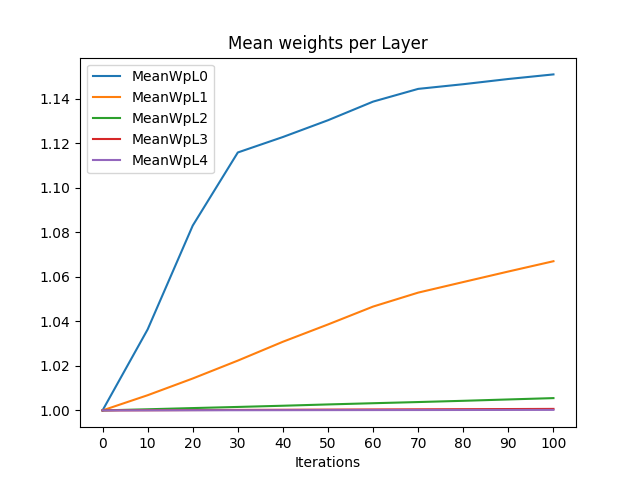
\includegraphics[width=1.1\linewidth]{images/plotA0_MeanWpL_AIDSPerfect_E_GDL_09_22h-03m}
				\caption{MeanWpL}
				\label{fig:plota0meanwplaidsperfectegdl0922h-03m}
			\end{subfigure}
			\begin{subfigure}{0.45\textwidth}
				\centering
				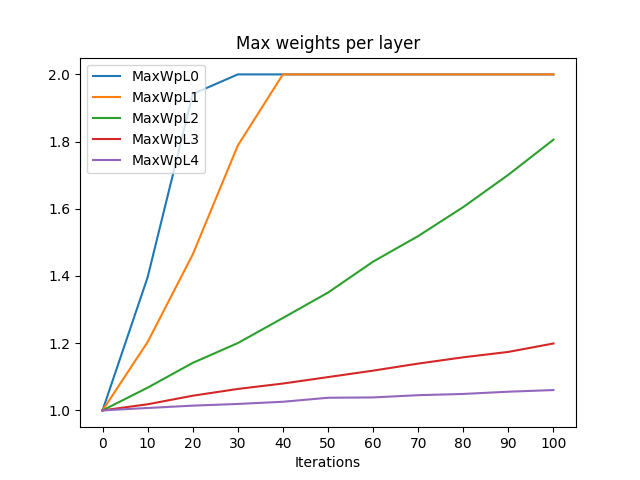
\includegraphics[width=1.1\linewidth]{images/plotA0_MaxWpL_AIDSPerfect_E_GDL_09_22h-03m}
				\caption{MaxWpL}
				\label{fig:plota0maxwplaidsperfectegdl0922h-03m}
			\end{subfigure}
			\caption{Mean and Maximum weight per layer - \textit{AIDS\_perfect}}
			\label{fig:MeanMaxWpLAIDSperfect}
		\end{figure}
	
		Notice how the limitation of the edge weights ($w\in[0,2]$) is visible in both graphs at around epoch $30$.
		In figure \ref{fig:plota0maxwplaidsperfectegdl0922h-03m} is visualized, how the maximum edge weights in the zeroth and first layer are no longer increased and stay at the maximum of $2.0$.
		In figure \ref{fig:plota0meanwplaidsperfectegdl0922h-03m} the growth of the average weights per layer is decreased afterwards.
		Recall, that the update rule allows to update edge weights with the same value in the same way.
		Thus these observations cannot be related to single edge weights in general.		
		
		The plots in figure \ref{fig:ClScoresAIDSperfect} show the evaluations on the Silhouette coefficient (SS), Davies-Bouldin score (DBS), and Calinski-Harabasz score (CHS).
		They reflect on the reached maximal edge weights as well.
		Up to epoch $20$ or $30$ they indicate an improvement. 
		After this, the cluster dispersion (caused by overall increasing weights) may be the reason for degenerating scores.
		
		\begin{figure}[H]
			\centering
			\begin{subfigure}{0.3\textwidth}
				\centering
				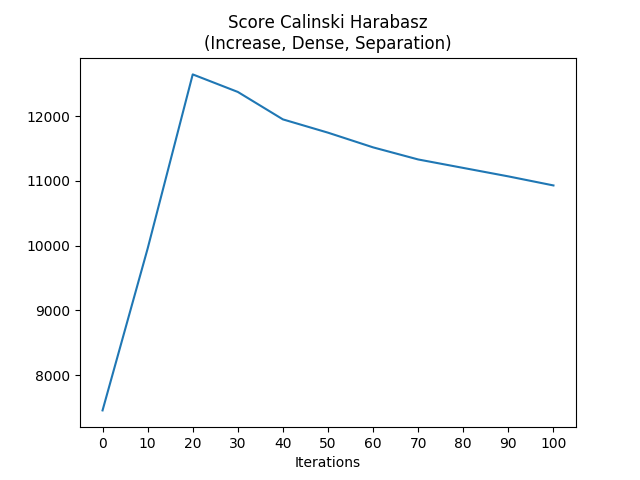
\includegraphics[width=1.1\linewidth]{images/plotA0_CHS_AIDSPerfect_E_GDL_09_22h-03m}
				\caption{CHS}
				\label{fig:plota0chsaidsperfectegdl0922h-03m}
			\end{subfigure}		
			\begin{subfigure}{0.3\textwidth}
				\centering
				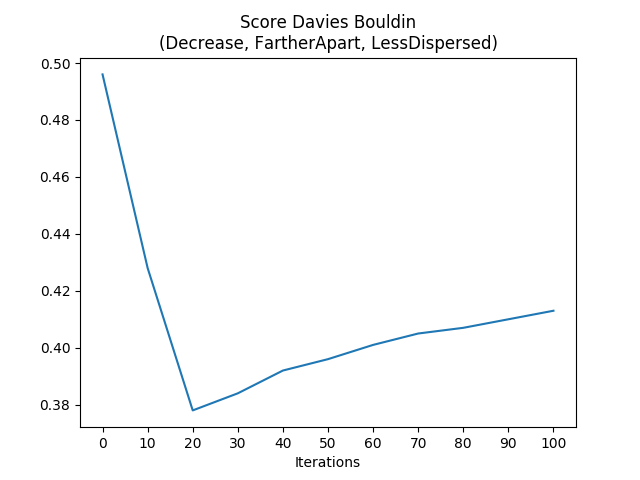
\includegraphics[width=1.1\linewidth]{images/plotA0_DBS_AIDSPerfect_E_GDL_09_22h-03m}
				\caption{DBS}
				\label{fig:plota0dbsaidsperfectegdl0922h-03m}
			\end{subfigure}
			\begin{subfigure}{0.3\textwidth}
				\centering
				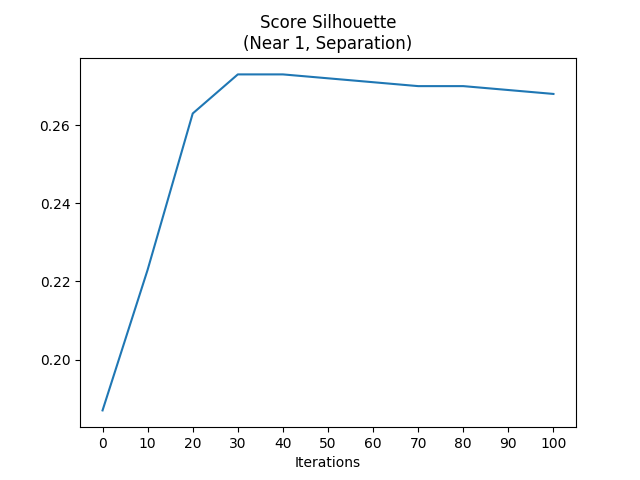
\includegraphics[width=1.1\linewidth]{images/plotA0_SS_AIDSPerfect_E_GDL_09_22h-03m}
				\caption{SS}
				\label{fig:plota0ssaidsperfectegdl0922h-03m}
			\end{subfigure}
			\caption{Cluster scores - \textit{AIDS\_perfect}}
			\label{fig:ClScoresAIDSperfect}
		\end{figure}
		
		A T-distributed Stochastic Neighbor Embedding (t-SNE)~\cite{2008_Maaten_CONF} visualizes the separation of the clusters in figure \ref{fig:TSNEAIDSperfect}.
		Overall, the clusters stay rather separated.
		An in- or decrease of the distance between them or the cluster denseness can not be noticed.
		However keep in mind, that the plots show a two-dimensional embedding of high dimensional (sparse) feature vectors.
		In this case, there are 34,296 WL-labels in the WLLT (with five layers $D=5$).
		Thus the feature vectors are 34,296-dimensional.
				
		\begin{figure}[H]
			\centering
			\begin{subfigure}{0.49\textwidth}
				\centering
				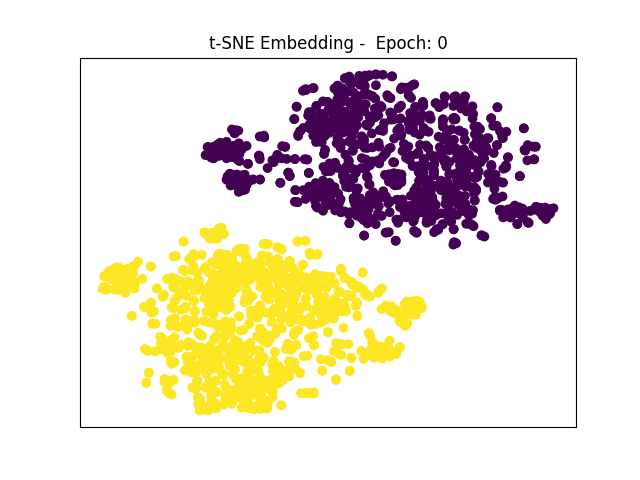
\includegraphics[width=1.1\linewidth]{images/plotA0_tSNE_e0_i0_AIDSPerfect_E_GDL_09_22h-03m}
				\caption{Epoch 0}
				\label{fig:plota0tsnee0i0aidsperfectegdl0922h-03m}
			\end{subfigure}
			\begin{subfigure}{0.49\textwidth}
				\centering
				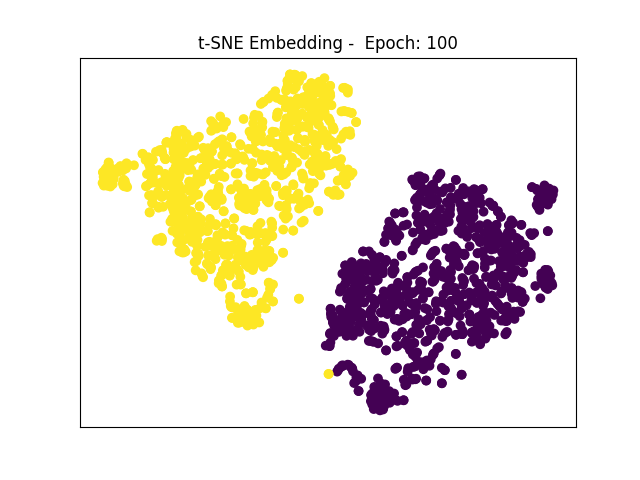
\includegraphics[width=1.1\linewidth]{images/plotA0_tSNE_e100_i10_AIDSPerfect_E_GDL_09_22h-03m}
				\caption{Epoch 100}
				\label{fig:plota0tsnee100i10aidsperfectegdl0922h-03m}
			\end{subfigure}
			\caption{T-SNE embeddings - \textit{AIDS\_perfect}}
			\label{fig:TSNEAIDSperfect}
		\end{figure}
		
		\begin{figure}[H]
			\centering
			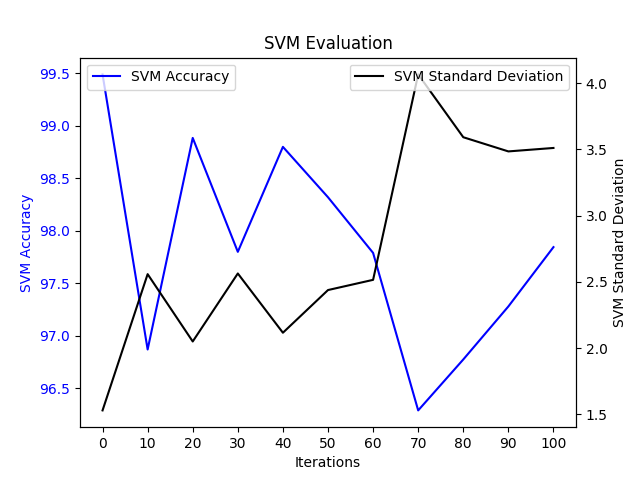
\includegraphics[width=0.7\linewidth]{images/plotA0_SVM_AIDSPerfect_E_GDL_09_22h-03m}
			\caption{SVM - \textit{AIDS\_perfect}}
			\label{fig:plota0svmaidsperfectegdl0922h-03m}
		\end{figure}		
	
		On the other hand figure \ref{fig:plota0svmaidsperfectegdl0922h-03m} illustrates that the SVM accuracy does not directly relate to these statistics.
		Overall, the SVM accuracy decreases and the best accuracy is reported for the initial state.
		This is indicates that the cluster scores and the SVM accuracy do not need improve or degenerate simultaneously.
		
		To summarize, this experiment supports the claim that the WLLT and the graph representations can be used in general to reflect a separation of graph clusters. 
		 	
	
	
	\subsubsection{Arbitrary Classifications} \label{subsubsec:exp_Arbitrary_Classifications} % Experiment 4
		In this experiment the learner was used two times with the same configuration.
		For one execution however, the classification for the graphs in the given dataset were randomized (keeping the number of classes). 
		The plots in figure \ref{fig:ArbitraryClCH} and \ref{fig:ArbitraryClSVM} show exemplary, that the learner behaves less predictable with respect to for example the CHS and the SVM accuracy.		
		Since the original classifications are related to the structures of the graph, but the randomized ones most likely not, this indicates that the learned edge weights do indeed capture information about the graph structures.
		
		\begin{figure}[H]
			\centering
			\begin{subfigure}{0.49\textwidth}
				\centering
				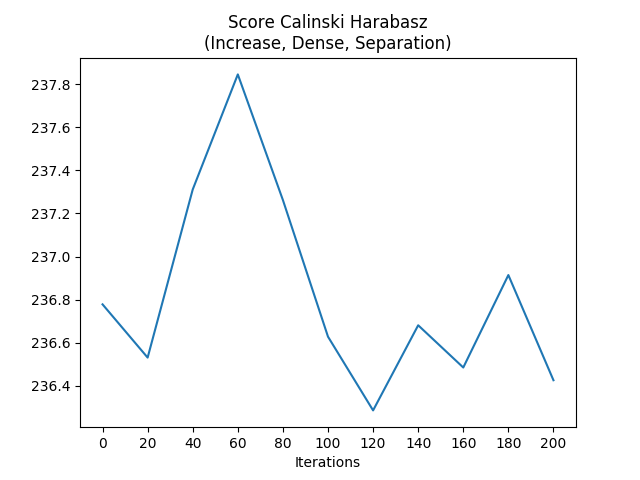
\includegraphics[width=1.1\linewidth]{images/plotE4_CH_E_GDL_09_16h-32m}
				\caption{Randomized classes}
				\label{fig:plote4chegdl0916h-32m}
			\end{subfigure}
			\begin{subfigure}{0.49\textwidth}
				\centering
				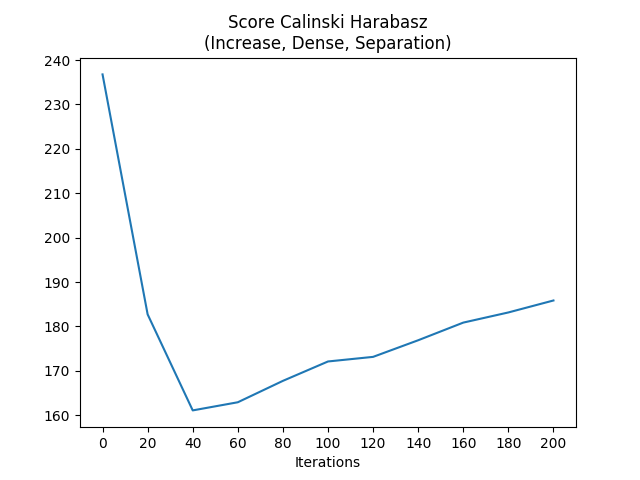
\includegraphics[width=1.1\linewidth]{images/plotE4_CH_E_GDL_09_17h-17m}
				\caption{Not randomized classes}
				\label{fig:plote4chegdl0917h-17m}
			\end{subfigure}
			\caption{CHS for the arbitrary classifications experiment - \textit{AIDS}}
			\label{fig:ArbitraryClCH}
		\end{figure}
		
		\begin{figure}[H]
			\centering
			\begin{subfigure}{0.49\textwidth}
				\centering
				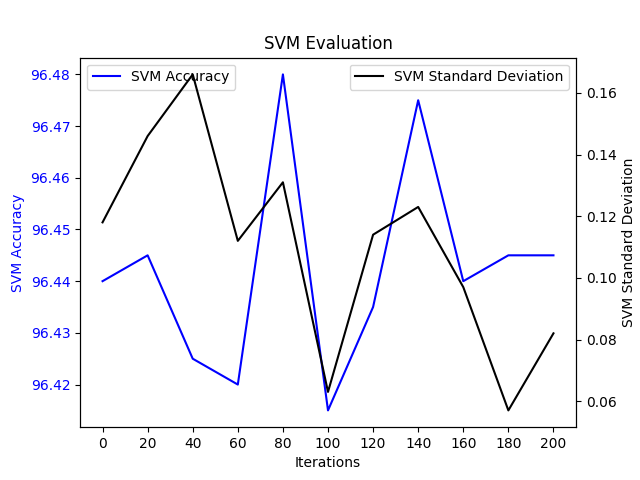
\includegraphics[width=1.1\linewidth]{images/plotE4_SVM_E_GDL_09_16h-32m}
				\caption{Randomized classes}
				\label{fig:fig:plote4svmegdl0916h-32m}
			\end{subfigure}
			\begin{subfigure}{0.49\textwidth}
				\centering
				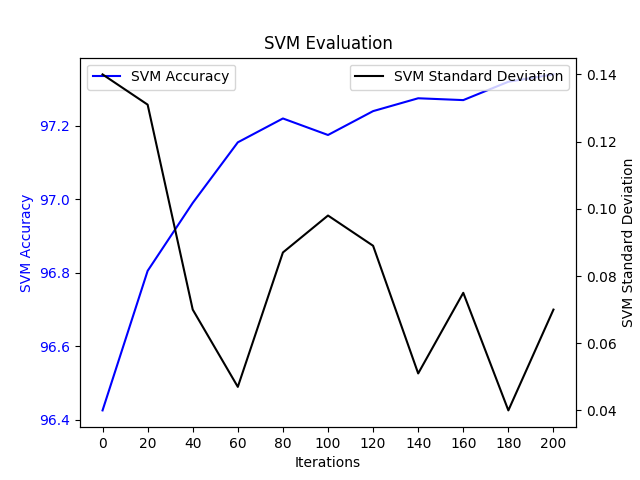
\includegraphics[width=1.1\linewidth]{images/plotE4_SVM_E_GDL_09_17h-17m}
				\caption{Not randomized classes}
				\label{fig:plote4svmegdl0917h-17m}
			\end{subfigure}
			\caption{SVM for the arbitrary classifications experiment - \textit{AIDS}}
			\label{fig:ArbitraryClSVM}
		\end{figure}
		
		Figure \ref{fig:WeightedWLLT} visualizes the WLLT with the learned edge weights.
		The plot in figure \ref{fig:plote4wlltl2e10gdl0917h-17mexp4} resembles a WLLT, typically for many of the conducted experiments.
		Plot \ref{fig:plote4wlltl2e10gdl0916h-32mexp4} on the other hand highlights how the learner has difficulties in defining meaningful weights for WL-labels and entire subtrees.
		
		\begin{figure}[H]
			\centering
			\begin{subfigure}{0.49\textwidth}
				\centering
				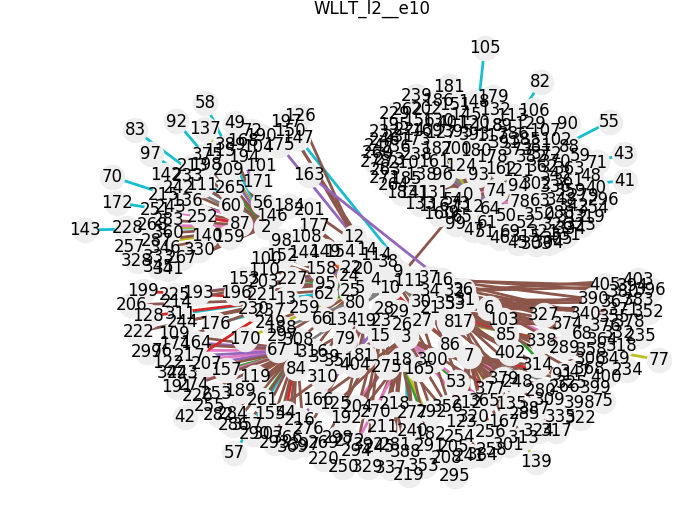
\includegraphics[width=1.1\linewidth]{images/plotE4_wllt_l2_e10_GDL_09_16h-32mExp4}
				\caption{Randomized classes}
				\label{fig:plote4wlltl2e10gdl0916h-32mexp4}
			\end{subfigure}
			\begin{subfigure}{0.49\textwidth}
				\centering
				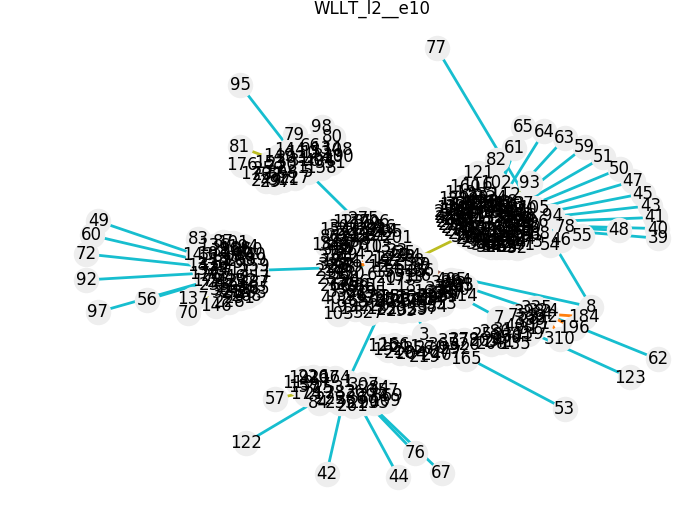
\includegraphics[width=1.1\linewidth]{images/plotE4_wllt_l2_e10_GDL_09_17h-17mExp4}
				\caption{Not randomized classes}
				\label{fig:plote4wlltl2e10gdl0917h-17mexp4}
			\end{subfigure}
			\caption{Weighted WLLT - \textit{AIDS}}
			\label{fig:WeightedWLLT}
		\end{figure}
	
		This experiment also indicates, that the l-WWLLT may not be able to learn arbitrary classifications in general.
		But this conclusion should be supported by more empirical or theoretical results.	

	\subsubsection{Relation between Pushing and Pulling} \label{subsubsec:exp_pp_factors}
		The success of the learning process seems to behave quite sensitively to the push and pull factors.
		This includes both their values and their relation between each other.
		Intuitively, if the pull factor is much greater than the push factor, the clusters collapse into each other and overlap.
		If on the other hand the push factor is much greater, the dispersion of the clusters increases which can lead to overlapping clusters as well.
		
		Researching the effect of these pp-factors and initializing them meaningfully becomes even more challenging, when different datasets are involved.
		Figure \ref{fig:plota4tsnee20enzymesgdl0418h} and \ref{fig:plota4tsnee0aids} show a t-SNE for the initialized l-WWLLT distances for the datasets \textit{ENZYMES} and \textit{AIDS} respectively.
		Notice how the different clusters overlap to different extends.
		
		\begin{figure}[H]
			\centering
			\begin{subfigure}{0.49\textwidth}
				\centering
				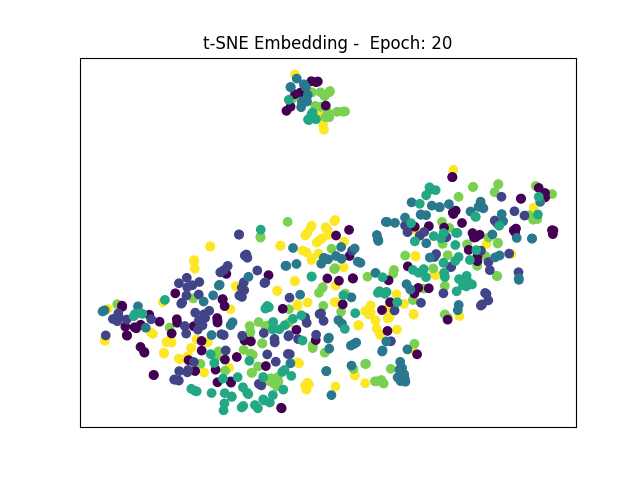
\includegraphics[width=1.1\linewidth]{images/plotA4_tSNE_e20_ENZYMES_GDL_04_18h-15m}
				\caption{\textit{ENZYMES}}
				\label{fig:plota4tsnee20enzymesgdl0418h}
			\end{subfigure}
			\begin{subfigure}{0.49\textwidth}
				\centering
				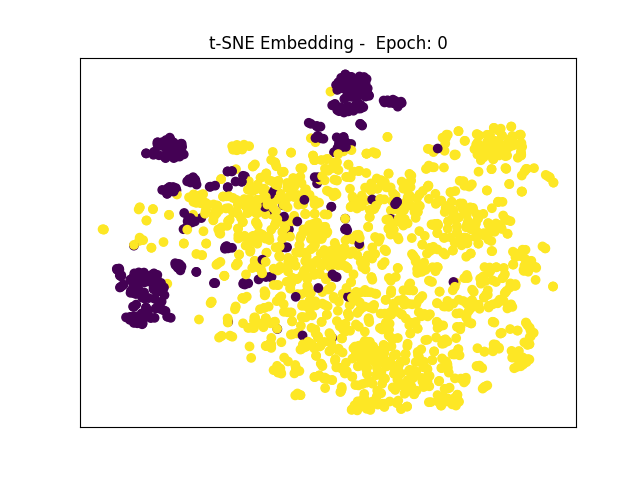
\includegraphics[width=1.1\linewidth]{images/plotA4_tSNE_e0_AIDS}
				\caption{\textit{AIDS}}
				\label{fig:plota4tsnee0aids}
			\end{subfigure}
			\caption{t-SNE of the uniformly initialized l-WWLLT}
			\label{fig:tSNE_init}
		\end{figure}
		
		The following four t-SNEs show the implied l-WWLLT distance after 100 learning epochs.
		In all configurations five WLLT layers were used.
		All except the first plot refer to the multiplicative update rule and a learning rate of $lr=1.0$.
		
		\begin{figure}[H]
			\centering
			\begin{subfigure}{0.49\textwidth}
				\centering
				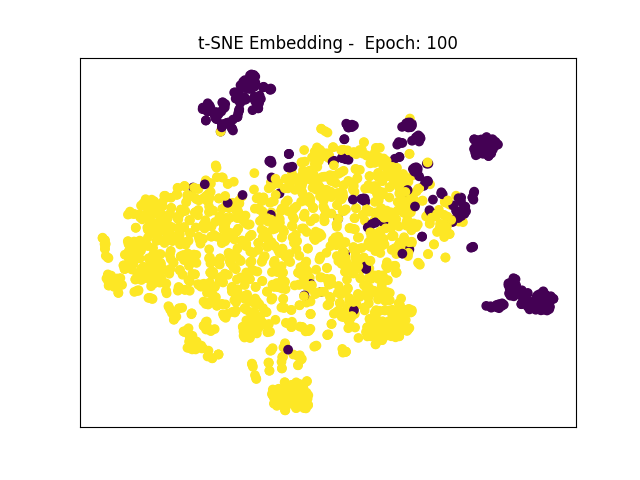
\includegraphics[width=1.1\linewidth]{images/plotA4_tSNE_e100_AIDS_E_GDL_18_23h-43m} % pp .3 lr .9
				\caption{pp-Factors: $0.3$, $lr=0.9$}
				\label{fig:plota4tsnee100aidsegdl1823h-43m}
			\end{subfigure}
			\begin{subfigure}{0.49\textwidth}
				\centering
				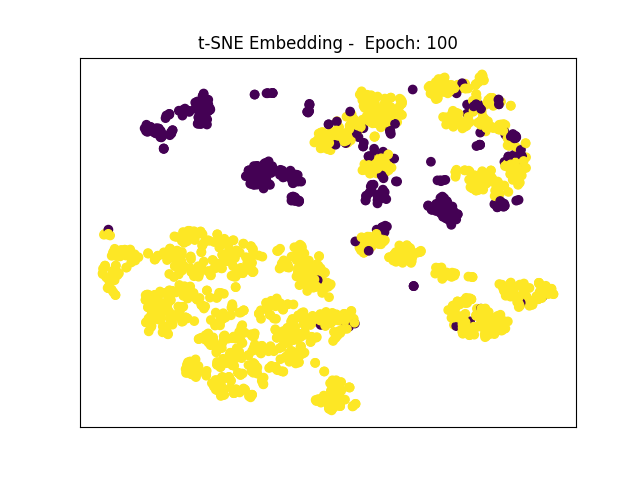
\includegraphics[width=1.1\linewidth]{images/plotA4_tSNE_e100_AIDS_E_GDL_24_17h-05m}  % pull.5push.5_noceil lr 1.0
				\caption{pp-Factors: $0.5$}
				\label{fig:plota4tsnee100aidsegdl2417h-05m}
			\end{subfigure}
			\caption{t-SNE of the l-WWLLT distances after $100$ epochs \& Equally strong push and pull factors - \textit{AIDS}}
			\label{fig:tSNE_100_A}
		\end{figure}
		
		Figure \ref{fig:plota4tsnee100aidsegdl1823h-43m} shows a configuration with $f_{\text{push}}=f_{\text{pull}}=0.3$ and $lr=0.9$.
		Almost no change to the initial state (figure \ref{fig:plota4tsnee0aids}) can be seen.
		One could argue that the clusters appear denser, but certainly not better separated.
		This may be, because the pp-factors, combined with the learning rate are to weak. 
		An example, where both are increased is shown in figure \ref{fig:plota4tsnee100aidsegdl2417h-05m}.
		Here the configuration $f_{\text{push}}=f_{\text{pull}}=0.5$ (and $lr=1.0$) was used.
		Again, the pp-factors are equally strong.
		Denser sub-clusters form in both clusters but the cluster separation remains weak.
		
		\begin{figure}[H]
			\centering
			\begin{subfigure}{0.49\textwidth}
				\centering
				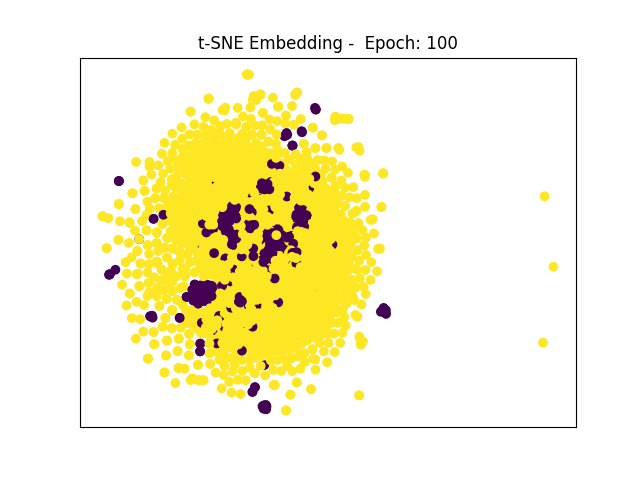
\includegraphics[width=1.1\linewidth]{images/plotA4_tSNE_e100_AIDS_E_GDL_24_12h-29m} % _pull.1 push.05 lr 1.0
				\caption{Pull: $0.1$, push: $0.05$}
				\label{fig:plota4tsnee100aidsegdl2412h-29m}
			\end{subfigure}
			\begin{subfigure}{0.49\textwidth}
				\centering
				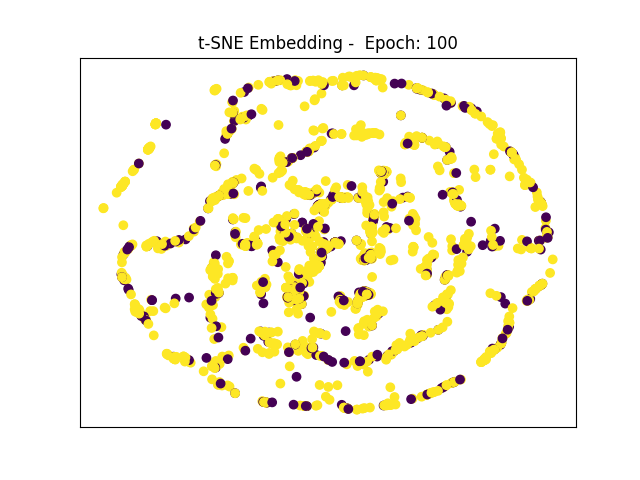
\includegraphics[width=1.1\linewidth]{images/plotA4_tSNE_e100_AIDS_E_GDL_24_13h-38m} % _pull.1 push.05 lr 1.0 absolute
				\caption{Pull: $0.1$, push: $0.05$ (additive update)}
				\label{fig:plota4tsnee100aidsegdl2413h-38m}
			\end{subfigure}
			\caption{t-SNE of the l-WWLLT distances after $100$ epochs \& Stronger pull. - \textit{AIDS}}
			\label{fig:tSNE_100_B}
		\end{figure}	
		
		Figure \ref{fig:plota4tsnee100aidsegdl2412h-29m} shows a configuration with unequal push and pull factors. 
		It is $f_{\text{push}}=0.05$ and $f_{\text{pull}}=0.1$.
		This is a good example for a typical case of heavily overlapping clusters because the pull factor is stronger that the push factor.
		
		Figure \ref{fig:plota4tsnee100aidsegdl2413h-38m} shows a configuration with $f_{\text{push}}=0.05$ and $f_{\text{pull}}=0.1$.
		Furthermore here, the pp-factors are used in the additive update rule.
		Interestingly the pull factor seems to pull again samples from both the same and different clusters together (compare to figure \ref{fig:plota4tsnee100aidsegdl2412h-29m}).
		However a significant separation is visible place at well.
		But such that the different clusters are separated.
		
		\begin{figure}[H]
			\centering
			\begin{subfigure}{0.49\textwidth}
				\centering
				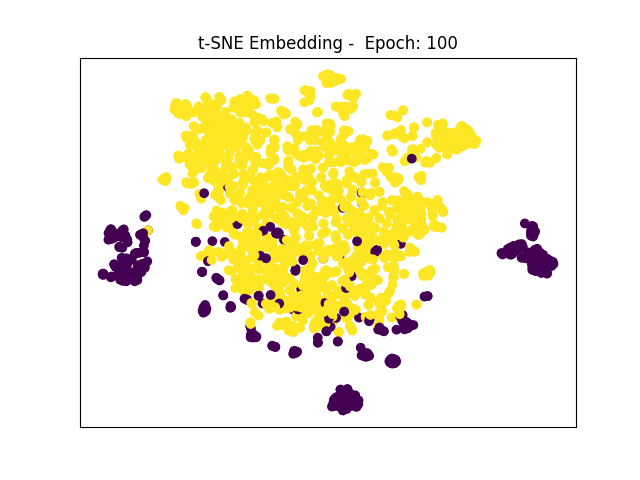
\includegraphics[width=1.1\linewidth]{images/plotA4_tSNE_e100_AIDS_E_GDL_09_01h_00m} %push 0.2 pull 0.1
				\caption{Pull: $0.1$, push: $0.2$}
				\label{fig:plota4tsnee100aidsegdl0901h00m}
			\end{subfigure}
			\begin{subfigure}{0.49\textwidth}
				\centering
				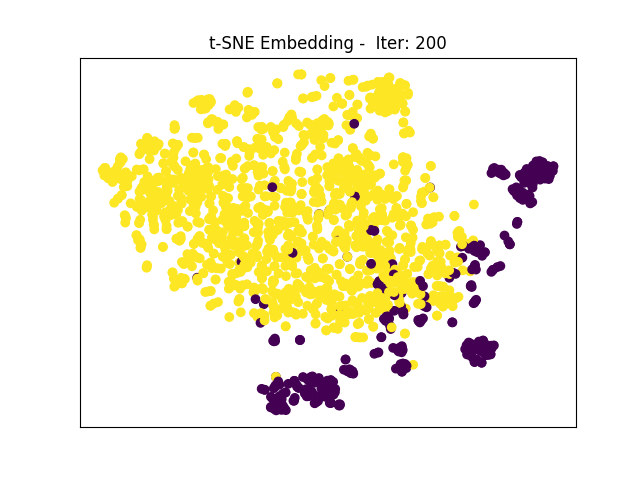
\includegraphics[width=1.1\linewidth]{images/plotA4_tSNE_e100_AIDS_E_GDL_03_02h-53m} %pull.1_psh.3
				\caption{Pull: $0.1$, push: $0.3$}
				\label{fig:plota4tsnee100aidsegdl0302h-53m}
			\end{subfigure}
			\caption{t-SNE of the l-WWLLT distances after $100$ epochs \& Stronger push - \textit{AIDS}}
			\label{fig:tSNE_100_C}
		\end{figure}
		
		Experiments, where the push factor is bigger than the pull factor tended to look like the original configuration, similar to figure \ref{fig:plota4tsnee100aidsegdl1823h-43m}
		again.
		Two examples of a common configuration from within a grid-search on the pp-Factors are visualized in figure \ref{fig:tSNE_100_C}.
		
		These exemplary plots do not cover the whole spectrum of the performed grid search. 
		But they shall give an insight on how different settings were perceived and that no clear trend could be established.
		Neither for all datasets, nor for one specifically.
		For further investigation, a more comprehensive grid search for the combination between pp-factors (and the learning rate) should be informative.	
	
	
%	\subsubsection{Single Layer Training} \label{subsubsec:exp_single_layer_training} % Experiment 5
%		The implementation allows to update edge weights of different layers differently.
%		So far, the other experiments do not motivate to use this.
%		For experimental variety however, a couple of experiments were conduced, such that only the edge weights of a single layer in the WLLT were updated.
%		Spot checks for different datasets and different WL layers did not show promising results.
%		While it was still possible to improve the cluster scores, the SVM performances were far behind the ones when updating all layers equally.
%		
%		%TODO: CONTINUE Exp5 of NCI1 or others. Plot where only one weight changes. Or delete this section.
%		
%		One may deduce from this, that the similarity of the graphs should be expressed as a matter of substructures of different sizes.
%		Since the WL-labels in layer $i$ only correspond to the i-1-th neighborhoods.
%		Adjusting the edge weights in different layers may allow to distinguish more accurately between variations in substructures of different sizes, which are relevant for the classification.
		
		
	\subsubsection{Dynamic PP-Factors} \label{subsubsec:exp_dynamic_pp} % Experiment 3
		So far all experiments are based on a fixed parameter configuration for all learning epochs.
		It is however a reasonable strategy, to dynamically change some of these parameters.
		For example by decreasing or increasing the learning rate, depending on the behavior of the error function.
		As mentioned before, the learning procedure is based purely on the local SME and does not consider the more expensive evaluations which were made after all learning epochs were completed.
		
		To investigate the effect of changing parameters, and to support the effectiveness of the implemented method, a set of experiments is based on the idea of continuing a given set of learning epochs with new learning parameters.
		We now consider a visually pleasing example on the dataset \textit{MSRC\_9}.
		400 learning epochs with parameters $D=4$, $lr=1.0$, $bs=0.3$, and $w\in[0,2]$ were performed.
		The first 200 epochs with a stronger pull, with $f_{\text{push}}=0.05$, $f_{\text{pull}}=0.3$.
		And the second 200 epochs with a stronger push, with $f_{\text{push}}=0.3$, $f_{\text{pull}}=0.05$.
		
		\begin{figure}[!ht]
			\centering
			\begin{subfigure}{0.49\textwidth}
				\centering
				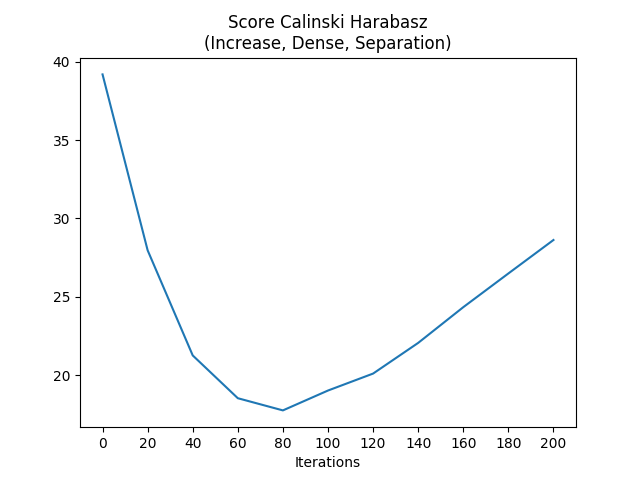
\includegraphics[width=1.1\linewidth]{images/plotE6_CHS_MSRC_9_E_GDL_22_00h-05mExp3pull}
				\caption{First 200 epochs}
				\label{fig:plote6chsmsrc9egdl2200h-05mexp3pull}
			\end{subfigure}
			\begin{subfigure}{0.49\textwidth}
				\centering
				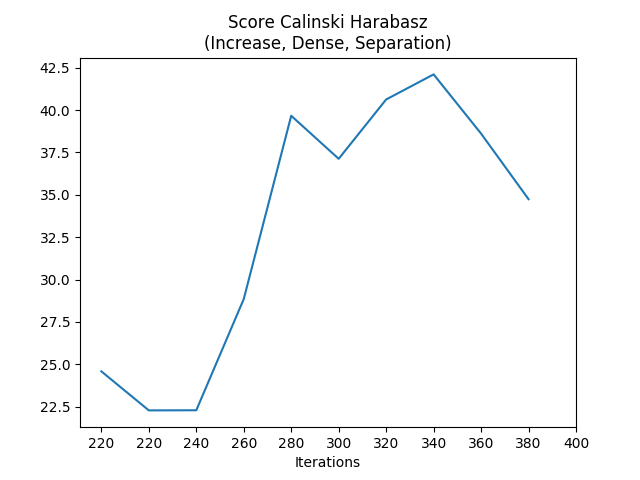
\includegraphics[width=1.1\linewidth]{images/plotE6_CHS_MSRC_9_E_GDL_22_00h-05mExp3pullpush}
				\caption{Second 200 epochs}
				\label{fig:plote6chsmsrc9egdl2200h-05mexp3pullpush}
			\end{subfigure}
			\caption{CHS - \textit{MSRC\_9}}
			\label{fig:E6CHS}
		\end{figure}
	
		\begin{figure}[!ht]
			\centering
			\begin{subfigure}{0.49\textwidth}
				\centering
				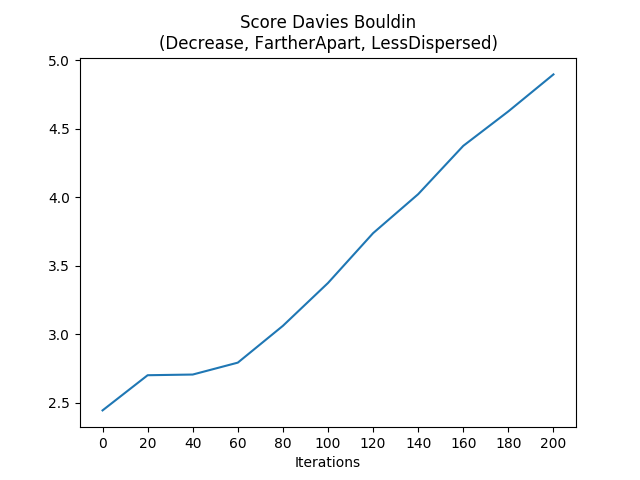
\includegraphics[width=1.1\linewidth]{images/plotE6_DBS_MSRC_9_E_GDL_22_00h-05mExp3pull}
				\caption{First 200 epochs}
				\label{fig:plote6dbsmsrc9egdl2200h-05mexp3pull}
			\end{subfigure}
			\begin{subfigure}{0.49\textwidth}
				\centering
				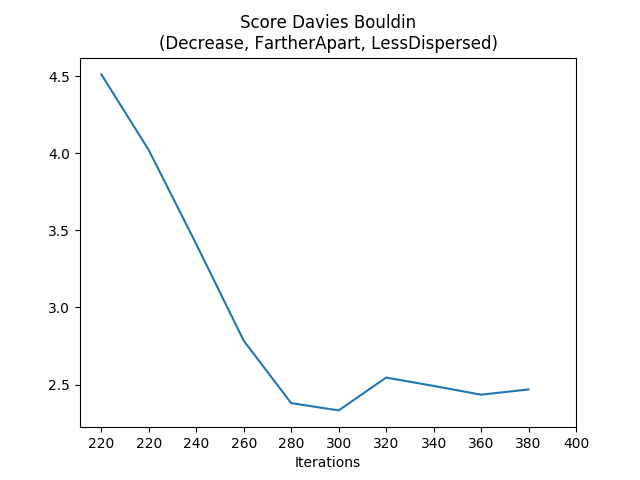
\includegraphics[width=1.1\linewidth]{images/plotE6_DBS_MSRC_9_E_GDL_22_00h-05mExp3pullpush}
				\caption{Second 200 epochs}
				\label{fig:plote6dbsmsrc9egdl2200h-05mexp3pullpush}
			\end{subfigure}
			\caption{DBS - \textit{MSRC\_9}}
			\label{fig:E6DBS}
		\end{figure}
	
		\begin{figure}[!ht]
			\centering
			\begin{subfigure}{0.49\textwidth}
				\centering
				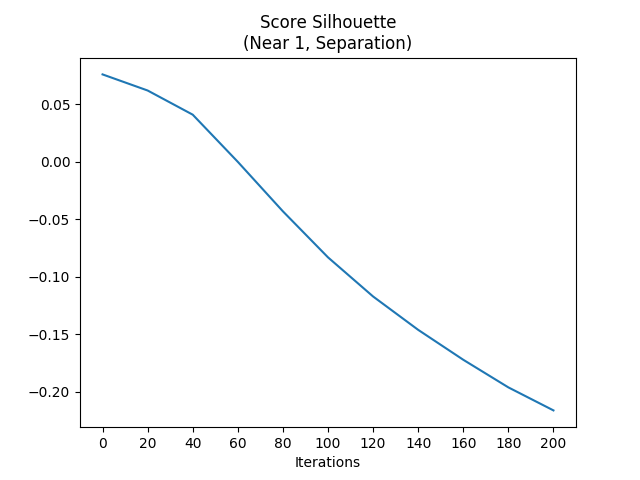
\includegraphics[width=1.1\linewidth]{images/plotE6_SS_MSRC_9_E_GDL_22_00h-05mExp3pull}
				\caption{First 200 epochs}
				\label{fig:plote6ssmsrc9egdl2200h-05mexp3pull}
			\end{subfigure}
			\begin{subfigure}{0.49\textwidth}
				\centering
				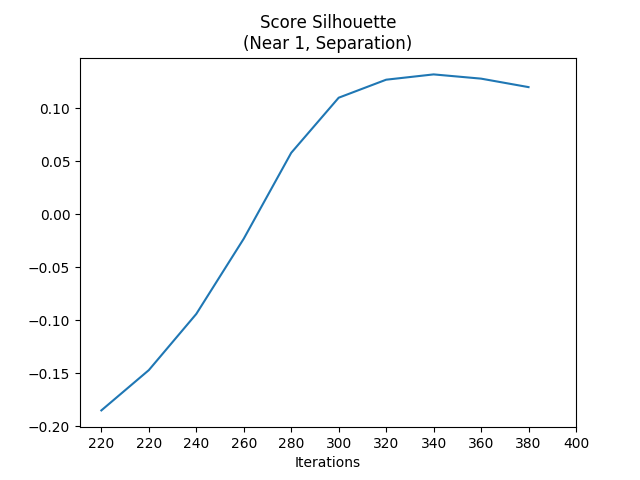
\includegraphics[width=1.1\linewidth]{images/plotE6_SS_MSRC_9_E_GDL_22_00h-05mExp3pullpush}
				\caption{Second 200 epochs}
				\label{fig:plote6ssmsrc9egdl2200h-05mexp3pullpush}
			\end{subfigure}
			\caption{SS - \textit{MSRC\_9}}
			\label{fig:E6SS}
		\end{figure}
	
		Figures \ref{fig:E6CHS}, \ref{fig:E6DBS} and \ref{fig:E6SS} clearly show, how the cluster scores are degenerating in the first 200 epochs, and improving in the last 200  epochs (or the last 180 in case of CHS).
		Figure \ref{fig:E6SVM} Shows the same behavior with respect to the SVM accuracy.
				
		\begin{figure}[!ht]
			\centering
			\begin{subfigure}{0.49\textwidth}
				\centering
				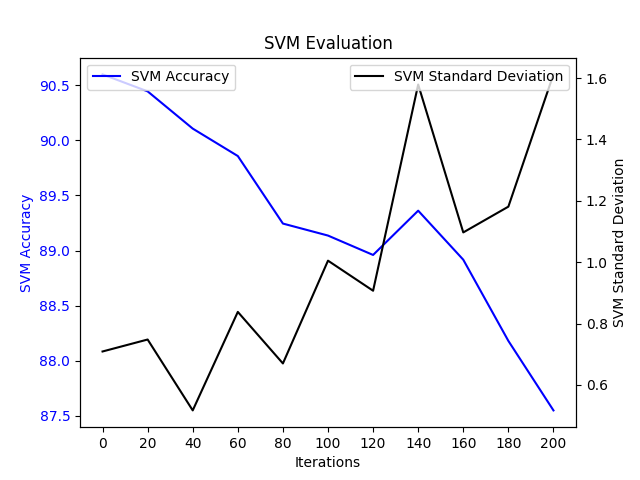
\includegraphics[width=1.1\linewidth]{images/plotE6_SVM_MSRC_9_E_GDL_22_00h-05mExp3pull}
				\caption{First 200 epochs}
				\label{fig:plote6svmmsrc9egdl2200h-05mexp3pull}
			\end{subfigure}
			\begin{subfigure}{0.49\textwidth}
				\centering
				\includegraphics[width=1.1\linewidth]{images/plotE6_SVM_MSRC_9_E_GDL_22_00h-05mExp3pullpush}
				\caption{Second 200 epochs}
				\label{fig:plote6svmmsrc9egdl2200h-05mexp3pullpush}
			\end{subfigure}
			\caption{SVM - \textit{MSRC\_9}}
			\label{fig:E6SVM}
		\end{figure}
		
		The t-SNEs in figure \ref{fig:E6tSNE1} and \ref{fig:E6tSNE2} support these findings too.
		Notice, that the uniform initialization of the WLLT edge weights already allows for a good SVM accuracy (figure \ref{fig:plote6svmmsrc9egdl2200h-05mexp3pull}) and dense, clearly separated clusters in the t-SNE (figure \ref{fig:plote6tsnee0msrc9egdl2200h-05mexp3pull}).
		The figures \ref{fig:plote6tsnee40msrc9egdl2200h-05mexp3pull} and \ref{fig:plote6tsnee100msrc9egdl2200h-05mexp3pull} are clear visualizations for the effects of the non-intuitive effects of a strong pull factor.
		The embeddings are clearly degenerating and same class samples are pushed apart, or at least the distances between all samples become less pronounced.
		On the other hand, the clustering is clearly improving in the second 200 epochs.
		One may discuss whether the clustering visualized in figure \ref{fig:plote6tsnee400msrc9egdl2200h-05mexp3pullpush} is better or worse than the original one in figure \ref{fig:plote6tsnee0msrc9egdl2200h-05mexp3pull}.
		Clearly, the clusters are less dense.
		Of all three cluster scores at least the CHS (figures \ref{fig:plote6chsmsrc9egdl2200h-05mexp3pullpush}) does support this observation, since the score at epoch 400 is worse than at epochs 0.
		Nevertheless this experiment clearly shows the strong effect of the pp-factors and their relation.
		Such experiments could be used to iteratively test parameter configurations in a sort of guided iterative grid search in future experiments.
				
		\begin{figure}[!ht]
			\centering
			\begin{subfigure}{0.3\textwidth}
				\centering
				\includegraphics[width=1.1\linewidth]{images/plotE6_tSNE_e0_MSRC_9_E_GDL_22_00h-05mExp3pull}
				\caption{Epoch 0}
				\label{fig:plote6tsnee0msrc9egdl2200h-05mexp3pull}
			\end{subfigure}		
			\begin{subfigure}{0.3\textwidth}
				\centering
				\includegraphics[width=1.1\linewidth]{images/plotE6_tSNE_e40_MSRC_9_E_GDL_22_00h-05mExp3pull}
				\caption{Epoch 40}
				\label{fig:plote6tsnee40msrc9egdl2200h-05mexp3pull}
			\end{subfigure}
			\begin{subfigure}{0.3\textwidth}
				\centering
				\includegraphics[width=1.1\linewidth]{images/plotE6_tSNE_e100_MSRC_9_E_GDL_22_00h-05mExp3pull}
				\caption{Epoch 100}
				\label{fig:plote6tsnee100msrc9egdl2200h-05mexp3pull}
			\end{subfigure}
			\caption{t-SNE - \textit{MSRC\_9}}
			\label{fig:E6tSNE1}
		\end{figure}
		
		\begin{figure}[!ht]
			\centering
			\begin{subfigure}{0.3\textwidth}
				\centering
				\includegraphics[width=1.1\linewidth]{images/plotE6_tSNE_e220_MSRC_9_E_GDL_22_00h-05mExp3pullpush}
				\caption{Epoch 220}
				\label{fig:plote6tsnee220msrc9egdl2200h-05mexp3pullpush}
			\end{subfigure}		
			\begin{subfigure}{0.3\textwidth}
				\centering
				\includegraphics[width=1.1\linewidth]{images/plotE6_tSNE_e280__MSRC_9_E_GDL_22_00h-05mExp3pullpush}
				\caption{Epoch 280}
				\label{fig:plote6tsnee280msrc9egdl2200h-05mexp3pullpush}
			\end{subfigure}
			\begin{subfigure}{0.3\textwidth}
				\centering
				\includegraphics[width=1.1\linewidth]{images/plotE6_tSNE_e400_MSRC_9_E_GDL_22_00h-05mExp3pullpush}
				\caption{Epoch 400}
				\label{fig:plote6tsnee400msrc9egdl2200h-05mexp3pullpush}
			\end{subfigure}
			\caption{t-SNE - \textit{MSRC\_9}}
			\label{fig:E6tSNE2}
		\end{figure}
		
		
	